% Options for packages loaded elsewhere
\PassOptionsToPackage{unicode}{hyperref}
\PassOptionsToPackage{hyphens}{url}
\PassOptionsToPackage{dvipsnames,svgnames*,x11names*}{xcolor}
%
\documentclass[
]{krantz}
\usepackage{amsmath,amssymb}
\usepackage{lmodern}
\usepackage{ifxetex,ifluatex}
\ifnum 0\ifxetex 1\fi\ifluatex 1\fi=0 % if pdftex
  \usepackage[T1]{fontenc}
  \usepackage[utf8]{inputenc}
  \usepackage{textcomp} % provide euro and other symbols
\else % if luatex or xetex
  \usepackage{unicode-math}
  \defaultfontfeatures{Scale=MatchLowercase}
  \defaultfontfeatures[\rmfamily]{Ligatures=TeX,Scale=1}
\fi
% Use upquote if available, for straight quotes in verbatim environments
\IfFileExists{upquote.sty}{\usepackage{upquote}}{}
\IfFileExists{microtype.sty}{% use microtype if available
  \usepackage[]{microtype}
  \UseMicrotypeSet[protrusion]{basicmath} % disable protrusion for tt fonts
}{}
\makeatletter
\@ifundefined{KOMAClassName}{% if non-KOMA class
  \IfFileExists{parskip.sty}{%
    \usepackage{parskip}
  }{% else
    \setlength{\parindent}{0pt}
    \setlength{\parskip}{6pt plus 2pt minus 1pt}}
}{% if KOMA class
  \KOMAoptions{parskip=half}}
\makeatother
\usepackage{xcolor}
\IfFileExists{xurl.sty}{\usepackage{xurl}}{} % add URL line breaks if available
\IfFileExists{bookmark.sty}{\usepackage{bookmark}}{\usepackage{hyperref}}
\hypersetup{
  pdftitle={``Deployando'' Bookdown: un flujo de trabajo como modelo de edición digital ramificada basada en estructuras descentralizadas, software libre y código abierto},
  pdfauthor={Andrés Lemos},
  colorlinks=true,
  linkcolor=Maroon,
  filecolor=Maroon,
  citecolor=Blue,
  urlcolor=Blue,
  pdfcreator={LaTeX via pandoc}}
\urlstyle{same} % disable monospaced font for URLs
\usepackage{longtable,booktabs,array}
\usepackage{calc} % for calculating minipage widths
% Correct order of tables after \paragraph or \subparagraph
\usepackage{etoolbox}
\makeatletter
\patchcmd\longtable{\par}{\if@noskipsec\mbox{}\fi\par}{}{}
\makeatother
% Allow footnotes in longtable head/foot
\IfFileExists{footnotehyper.sty}{\usepackage{footnotehyper}}{\usepackage{footnote}}
\makesavenoteenv{longtable}
\usepackage{graphicx}
\makeatletter
\def\maxwidth{\ifdim\Gin@nat@width>\linewidth\linewidth\else\Gin@nat@width\fi}
\def\maxheight{\ifdim\Gin@nat@height>\textheight\textheight\else\Gin@nat@height\fi}
\makeatother
% Scale images if necessary, so that they will not overflow the page
% margins by default, and it is still possible to overwrite the defaults
% using explicit options in \includegraphics[width, height, ...]{}
\setkeys{Gin}{width=\maxwidth,height=\maxheight,keepaspectratio}
% Set default figure placement to htbp
\makeatletter
\def\fps@figure{htbp}
\makeatother
% Make links footnotes instead of hotlinks:
\DeclareRobustCommand{\href}[2]{#2\footnote{\url{#1}}}
\setlength{\emergencystretch}{3em} % prevent overfull lines
\providecommand{\tightlist}{%
  \setlength{\itemsep}{0pt}\setlength{\parskip}{0pt}}
\setcounter{secnumdepth}{5}
\usepackage{booktabs}
\ifluatex
  \usepackage{selnolig}  % disable illegal ligatures
\fi
\usepackage[]{natbib}
\bibliographystyle{apalike}

\title{``Deployando'' Bookdown: un flujo de trabajo como modelo de edición digital ramificada basada en estructuras descentralizadas, software libre y código abierto}
\author{Andrés Lemos}
\date{Febrero de 2022}

\begin{document}
\maketitle

{
\hypersetup{linkcolor=}
\setcounter{tocdepth}{1}
\tableofcontents
}
\hypertarget{section}{%
\chapter*{\textgreater{}}\label{section}}



\includegraphics{images/portada.png}

\hypertarget{licencias}{%
\chapter*{Licencia de Producción de Pares (versión legible por humanes)}\label{licencias}}


\begin{quote}
Esto es un resumen legible por humanos del \href{http://endefensadelsl.org/ppl_es.html}{texto legal (la licencia
completa)}
\#\# Ud. es libre de \{-\}
\end{quote}

\begin{itemize}
\tightlist
\item
  Compartir - copiar, distribuir, ejecutar y comunicar públicamente la obra
\item
  Hacer obras derivadas
\end{itemize}

\hypertarget{bajo-las-condiciones-siguientes}{%
\section*{Bajo las condiciones siguientes:}\label{bajo-las-condiciones-siguientes}}


\begin{figure}
\centering

\includegraphics{images/by.png}
\caption{\textbf{Atribución} - Debe reconocer los créditos de la obra de la manera
especificada por el autor o el licenciante (pero no de una manera que sugiera
que tiene su apoyo o que apoyan el uso que hace de su obra).}
\end{figure}

\begin{figure}
\centering

\includegraphics{images/sa.png}
\caption{\textbf{Compartir bajo la Misma Licencia} - Si altera o transforma esta obra, o
genera una obra derivada, sólo puede distribuir la obra generada bajo una
licencia idéntica a ésta.}
\end{figure}

\begin{figure}
\centering

\includegraphics{images/nc.png}
\caption{\textbf{No Capitalista} - La explotación comercial de esta obra sólo está permitida
a cooperativas, organizaciones y colectivos sin fines de lucro, a
organizaciones de trabajadores autogestionados, y donde no existan relaciones
de explotación. Todo excedente o plusvalía obtenidos por el ejercicio de los
derechos concedidos por esta Licencia sobre la Obra deben ser distribuidos por y
entre los trabajadores.}
\end{figure}

\hypertarget{entendiendo-que}{%
\section*{Entendiendo que}\label{entendiendo-que}}


\begin{itemize}
\item
  \textbf{Renuncia} - Alguna de estas condiciones puede no aplicarse si se obtiene
  el permiso del titular de los derechos de autor.
\item
  \textbf{Dominio Público} - Cuando la obra o alguno de sus elementos se halle en
  el dominio público según la ley vigente aplicable, esta situación no quedará
  afectada por la licencia.
\item
  \textbf{Otros derechos} - Los derechos siguientes no quedan afectados por
  la licencia de ninguna manera:

  \begin{itemize}
  \item
    Los derechos derivados de usos legítimos u otras limitaciones
    reconocidas por ley no se ven afectados por lo anterior;
  \item
    Los derechos morales del autor;
  \item
    Derechos que pueden ostentar otras personas sobre la propia obra o
    su uso, como por ejemplo derechos de imagen o de privacidad.
  \end{itemize}
\item
  \textbf{Aviso} - Al reutilizar o distribuir la obra, tiene que dejar muy en cla
  los términos de la licencia de esta obra. La mejor forma de hacerlo es
  enlazar a esta página.
\end{itemize}

\hypertarget{intro}{%
\chapter{\texorpdfstring{Introducción: \emph{Bookdown} como herramienta de publicación ramificada}{Introducción: Bookdown como herramienta de publicación ramificada}}\label{intro}}

El flujo de trabajo que se propone a continuación, así como la composición, imposición y archivos digitales de este TPF, fueron realizados con herramientas de código abierto y de uso gratuito\footnote{Para acceder a la versión web y demás formatos de salida de este trabajo, visitar: \url{https://etalii.github.io/tepepub/}}; principalmente \emph{Bookdown}, \emph{GitHub} y \emph{Zotero}. El objetivo de este trabajo es explicar y documentar el desarrollo de un proyecto editorial que combina dichas herramientas en un flujo de trabajo basado en software libre y de acceso abierto, y que se orienta hacia un esquema de edición digital ramificada, descentralizada y distribuida.

Así, los métodos propuestos en este trabajo se organizan en un flujo editorial ramificado \citep{ramiroEdicionDigitalComo2018} que consta de tres grandes etapas: componer, compilar y publicar (ver Figura \ref{fig:workflow} ). A grandes rasgos y a los efectos de este desarrollo, componer se refiere a producir los archivos fuente y darles formato en R \href{https://es.wikipedia.org/wiki/Markdown}{Markdown}, la versión del lenguaje de marcado \emph{Markdown} optimizada para el lenguaje de programación \emph{R}; compilar consiste en correr un conjunto de comandos, funciones y fragmento de código de \emph{R} para imponer y generar los archivos de salida; mientras que publicar consiste en la disposición pública de la publicación en alguna plataforma y/o soporte.

Es decir que, la técnica productiva y reproductiva \citep{seminariopublicacionesdigitalesUnidadParte2021} que se presenta en este desarrollo se organiza mediante un flujo de trabajo, cuya característica es combinar una serie de scripts, algoritmos y metadatos, de forma que un mismo contenido se adapte a distintos tipos de publicaciones, productos digitales e incluso, publicaciones impresas. Una consecuencia de esta característica es que en un solo paso se generan múltiples archivos y publicaciones digitales para distintos propósitos, dispositivos y plataformas:

\begin{itemize}
\tightlist
\item
  Archivo del código fuente de la publicación en formato de extensión .md (\emph{Markdown}) completo con rutas de acceso a imágenes estáticas para una fácil conversión a la plataforma del editor.
\item
  Edición web HMTL para el libro de acceso abierto, con \emph{iframes} integrados a gráficos, videos, \emph{gifs} y mapas interactivos.
\item
  Edición impuesta para imprenta (original de pre-prensa), lectura digital en formato PDF enriquecido.
\item
  Edición en formato EPUB de acceso abierto, con \emph{iframes} integrados a gráficos, videos, \emph{gifs} y mapas interactivos.
\item
  Edición en formatos de extensión .doc (Microsoft Word) y .odt (Libreoffice) para obras derivadas, revisiones y comentarios.
\end{itemize}

Entonces, a diferencia de lo que ocurre en un flujo de trabajo editorial de tipo lineal, que requiere de la creación de archivos y códigos distintos para diferentes tipos de ediciones y publicaciones; en el esquema del flujo de trabajo ramificado, la producción de los originales, el seguimiento del proceso editorial, la revisión, la corrección, las colaboraciones y el control de cambios, ocurren todos sobre un mismo archivo y de forma paralela.

Todo esto a su vez se relaciona con determinados modos de editar (colaborativos y descentralizados), formas de poner el contenido en los soportes (líquida, abierta y distribuida), y las estrategias comerciales y de promoción de ventas.



\begin{figure}

{\centering 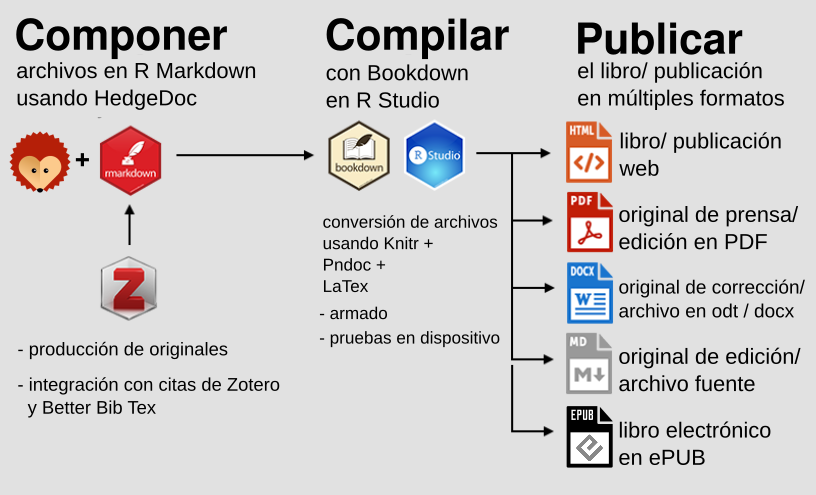
\includegraphics[width=0.8\linewidth]{images/workflow} 

}

\caption{Esquema simplificado de las etapas generales del flujo de trabajo, componer, compilar y publicar en múltiples formatos}\label{fig:workflow}
\end{figure}

\hypertarget{sobre-bookdown-extensiones-y-software-complementario}{%
\section{\texorpdfstring{Sobre \emph{Bookdown}, extensiones y software complementario}{Sobre Bookdown, extensiones y software complementario}}\label{sobre-bookdown-extensiones-y-software-complementario}}

El flujo de trabajo está desarrollado en \href{https://bookdown.org}{Bookdown}, un paquete de código abierto para el lenguaje de programación \href{https://www.r-project.org/}{R}, creado por Yihui Xie para la aplicación de escritorio gratuita \href{https://rstudio.com/}{RStudio}. Aunque mucha gente usa \emph{R} para análisis estadístico, \emph{RStudio} también es compatible con varias soluciones de publicación ramificada. Así, los pasos que forman parte de las tres grandes etapas (componer, compilar y publicar) de este flujo de trabajo estan determinadas por \emph{Bookdown}:

\begin{enumerate}
\def\labelenumi{\arabic{enumi}.}
\tightlist
\item
  Durante la etapa de composición:
\end{enumerate}

\begin{itemize}
\item
  Configuración de los archivos de \emph{Bookdown} de forma que cada capítulo/ sección conste de un archivo de \emph{R Markdown} (extensión .Rmd).
\item
  Organización de las citas, fuentes y referencias utilizando el gestor bibliográfico \href{https://zotero.org/}{Zotero} desarrollado por el \href{https://rrchnm.org/}{Centro Roy Rosenzweig de Historia y Nuevos Medios de la Universidad George Mason}. Además, hay que instalar la extensión \href{https://github.com/retorquere/zotero-better-bibtex}{Better BibTeX} para crear claves de citas en \emph{Zotero} compatibles con \emph{Bookdown}.
\end{itemize}

\begin{enumerate}
\def\labelenumi{\arabic{enumi}.}
\setcounter{enumi}{1}
\tightlist
\item
  Durante la etapa de compilación:
\end{enumerate}

\begin{itemize}
\item
  Creación de los archivos de salida utilizando el conversor universal de documentos \href{https://pandoc.org/}{PanDoc} y el software de preparación de documentos \href{https://www.latex-project.org/}{LaTeX}.
\item
  Configuración de los datos de identificación en fuente y la capa de \protect\hyperlink{licencias}{licenciamiento} libre (\emph{copyleft}) o abierto (\emph{Creative Commons}) en el archivo \texttt{index.Rmd} mediante una plantilla específica que se compila con el original.
\item
  Definición diferencial de contenido en función del formato de salida usando fragmentos de código de \emph{R}. Esto se puede hacer incluso durante el proceso de escritura para hacer publicaciones parciales, generar capítulos promocionales, desarrollar la audiencia y hasta abrir la posibilidad de incorporar comentarios de lectorxs y colaboradores. Con las revisiones de cada jornada de trabajo se puede recompilar el libro, publicar las ediciones en el repositorio público de \emph{GitHub} y usar el \href{https://pages.github.com/}{generador de sitios estáticos integrado} para alojar el formato web HTML de la publicación (libro/ publicación web).
\end{itemize}

\begin{enumerate}
\def\labelenumi{\arabic{enumi}.}
\setcounter{enumi}{2}
\tightlist
\item
  Durante la etapa de publicación:
\end{enumerate}

\begin{itemize}
\item
  Subida de los archivos fuente a un repositorio de \href{https://github.com/}{\emph{GitHub}} (repo), que además de hacer posible la disposición pública de la publicación en internet mediante un sitio web; permite al equipo editorial, conocer las versiones del texto que se generan (traducción, corrección, revisión, ramificación, reedición, erc), planificar el proyecto, seguir el desarrollo del proceso editorial y a los autores, trabajar simultáneamente en el libro/ publicación en un repositorio común\^{}{[}Para acceder al repositorio de \emph{GitHub} de este trabajo a modo de ejemplo, visitar: \url{https://github.com/etalii/tepepub}).
\item
  Implementar el modelo de \href{https://docs.microsoft.com/es-es/devops/deliver/what-is-infrastructure-as-code}{infraestructura como código} para alojar el libro/ publicación web gratuitamente mediante \emph{GitHub pages} (hosting). De esta forma, el sitio web que se genera, no solamente funciona como un producto editorial en sí, sino que además puede funcionar como interfaz de acceso al resto de las versiones de la publicación o ediciones (pdf, epub, mobi ,docx y md).
\end{itemize}

Sin embargo, la descripción del flujo de trabajo desarrollado en \emph{Bookdown} que se hace aquí, no es exhaustiva y comprende solo un conjunto de elementos de análisis pertinentes a los contenidos del Seminario de Publicaciones Digitales. Para obtener más detalles técnicos sobre \emph{Bookdown} y ejemplos de otras publicaciones creadas con esta herramienta, se puede consultar \url{https://bookdown.org} \footnote{- Xie, Yihui. Bookdown: Authoring Books and Technical Documents with R Markdown. Chapman \& Hall/CRC, 2018. \url{https://bookdown.org/yihui/bookdown/}. - Xie, Yihui, J. J. Allaire, and Garrett Grolemund. R Markdown: The Definitive Guide. Chapman \& Hall/CRC, 2020. \url{https://bookdown.org/yihui/rmarkdown/}. - Xie, Yihui, Christophe Dervieux, and Emily Riederer. R Markdown Cookbook. Chapman \& Hall/CRC, 2020. \url{https://bookdown.org/yihui/rmarkdown-cookbook/}.}.

\hypertarget{cuxf3mo-instalar-y-configurar-bookdown}{%
\section{\texorpdfstring{Cómo instalar y configurar \emph{Bookdown}}{Cómo instalar y configurar Bookdown}}\label{cuxf3mo-instalar-y-configurar-bookdown}}

A continuación, se enumeran los pasos que hay que seguir para configurar la plataforma de publicación (\emph{Bookdown}) y las herramientas relacionadas necesarias para compilar este trabajo, utilizando \emph{Ubuntu 20.04}. Esto no requiere conocimientos especiales sobre \emph{Linux}, de forma que los pasos para la instalación y la configuración en \emph{Ubuntu}, si bien son diferentes, son similares a los que se deben seguir para \emph{Windows} y \emph{MacOs}.

\begin{enumerate}
\def\labelenumi{\arabic{enumi}.}
\item
  Instalar el lenguaje de programación \emph{R}, requerido para usar \emph{Bookdown}.
\item
  Instalar la versión gratuita de \emph{RStudio Desktop} para facilitar el uso de \emph{R} mediante la interfaz gráfica del editor de texto. Algunes autores componen sus textos directo en \emph{RStudio}, pero es recomendable usar algún editor de texto (como \href{https://docutopia.tupale.co/}{HedgeDoc} ), ya que estos suelen tener comandos, atajos y opciones específicas que hacen más ágil la escritura.
\item
  Dentro de \emph{RStudio}, dirigirse a la pestaña `` \emph{Packages} '' y seleccionar `` \emph{Install} '' ( \href{images/packages-install.png}{ver captura de pantalla} ).
\item
  Dentro de \emph{RStudio}, instalar el paquete " \emph{bookdown} " y seleccionar `` \emph{Install Dependencies} '' ( \href{images/bookdown-install.png}{ver captura de pantalla} ).
\item
  Para que \emph{Bookdown} cree la versión de la publicación en PDF hay que instalar un motor de \href{https://en.wikipedia.org/wiki/LaTeX}{LaTeX} que transforme los formatos de las citas e imágenes de \emph{Markdown} a estilos de página preconfigurados. Dado que \emph{LaTeX} es muy pesado, la documentación de \emph{Bookdown} recomienda el paquete \emph{TinyTeX} que es más ligero. Para instalarlo, dentro de \emph{RStudio} hay que seleccionar la pestaña `` \emph{Packages} '', seleccionar `` \emph{Install} '' y tipear " \emph{tinytex} " para buscar y cargar el paquete ( \href{images/tinytex-install.png}{ver captura de pantalla} ).
\item
  Para terminar de instalar " \emph{tinytex} " hay que escribir \texttt{tinytex\ ::\ install\_tinytex\ ()} en la consola de RStudio y presionar `` \emph{return} ''. ( \href{images/tinytex-finish.png}{ver captura de pantalla} )
\item
  Junto con la instalación de \emph{RStudio}, hay que instalar \emph{Pandoc}, el paquete que convierte archivos del formato \emph{Markdown} a HMTL y otros formatos. Para confirmar la instalación de \emph{Pandoc} y el número de versión hay que escribir \texttt{rmarkdown\ ::\ pandoc\_version\ ()} en la consola de \emph{RStudio}, y presionar `` \emph{return} ''. El número de la versión instalada debe ser 2.3.1 o superior. Para instalar una versión más reciente de \emph{Pandoc}, que es muy recomendable, dirigirse a \url{https://pandoc.org}.
\end{enumerate}

\hypertarget{componer}{%
\chapter{Componer}\label{componer}}

\hypertarget{estructura-de-archivos-y-encabezados}{%
\section{Estructura de archivos y encabezados}\label{estructura-de-archivos-y-encabezados}}

En general, cada capítulo es un archivo .Rmd independiente. Esto implica que, en caso de editar el contenido de la publicación en simultáneo, les coautorxs tienen que trabajar en diferentes capítulos del libro y enviar regularmente \emph{commits} al repositorio. Una alternativa para evitar conflictos en el repositorio, es trasladar el proceso de escritura a un editor de texto externo especializado en \emph{Markdown} que tenga control de versiones, que sea colaborativo y multiplataforma, como \emph{HedgeDoc}. Del mismo modo, es recomendable que solamente une miembrx del equipo compile regularmente el libro con \emph{Bookdown} para evitar conflictos de combinación de código.

A continuación se propone un esquema simplificado de la estructura del archivo raíz del proyecto (y disponible en el repositorio de \emph{GitHub}):

\begin{itemize}
\item
  Prefacio de la publicación con secciones no numeradas: \texttt{index.Rmd}
\item
  Capítulos con encabezados de primer nivel en este formato: \texttt{01-capitulo.Rmd}
\item
  Secciones dentro de los capítulos con encabezados de segundo nivel en este formato: \texttt{01.1-subcapítulo.Rmd}.
\item
  La carpeta de imágenes, donde se encuentran las imágenes PNG, JPG y PDF que se van a renderizar y mostrar en los capítulos.
\item
  La carpeta \emph{docs}, que contiene los archivos fuente de la publicación, como la edición Web (\texttt{index.html}, \texttt{Introduccion.html}, etc.), la salida PDF, etc.
\item
  Archivos auxiliares adicionales que se describen más adelante.
\end{itemize}

Una forma que ofrece \emph{Bookdown} para manejar las referencias cruzadas es la asignación de un ID predeterminado a cada encabezado. Por ejemplo, el ID predeterminado para \texttt{\#\ Tema} es \texttt{\{\#tema\}}, y el ID predeterminado para \texttt{\#\#\ Nombre\ de\ sección} es \texttt{\{\#\ nombre-de-sección\}}, donde los espacios se reemplazan por guiones.

Como los IDs predeterminados pueden cambiar debido a la edición o estar duplicados en la publicación, en su lugar se puede asignar manualmente un ID único a cada encabezado de primer y segundo nivel de la siguiente manera:

\begin{verbatim}
# Título de capítulo de primer nivel de jerarquía {#nombre-único}
## Título de sección de segundo nivel de jerarquía {- #nombre-único}
### Título de sección de tercer nivel de jerarquía {-}
#### Título de sección de cuarto nivel de jerarquía {-}
\end{verbatim}

De forma que es importante tener en cuenta que el símbolo \{-\}, usado solo o en combinación con un espacio y una identificación única, evita la numeración automática en los encabezados de segundo a cuarto nivel.

Además, es posible hacer coincidir la palabra clave ID única con el nombre del archivo para los capítulos de nivel superior de esta manera: \texttt{01-palabra-clave.Rmd} para mayor organización. Los nombres únicos deben contener solamente caracteres alfanuméricos (a-z, A-Z, 0-9) o guiones (-). A su vez, los subtítulos deben tener nombres o IDs únicos para evitar errores de \emph{Bookdown} sobre referencias duplicadas. Para evitar este problema con los subtítulos repetidos (como podría darse en el uso de una sección ``Resumen''), al final de cada capítulo se puede insertar un subtítulo de resumen de tercer nivel, pero para eso hay que usar un ID único que coincida con el número de cada capítulo, como este: \texttt{\#\#\#\ Resumen\ \{-\ \#\ resumen17\}}. Del mismo modo, un encabezado especial podría constituir por ejemplo, un apéndice e indicarse con \texttt{(APÉNDICE)}. indicando que todos los capítulos que aparecen después son apéndices. Según la documentación de \emph{Bookdown}, el estilo de numeración aparecerá correctamente en la salida HTML y LaTeX / PDF, pero no en .doc y otros formatos de libros / publicaciones electrónicos.

\begin{verbatim}
# Capítulo Uno

# Capítulo Dos

# (APÉNDICE) Apéndice {-}

# Apéndice A

# Apéndice B
\end{verbatim}

Por otro lado, en el archivo \texttt{index.Rmd} del directorio de trabajo del proyecto se configuran las opciones para la salida del libro/ publicación HTML y la salida PDF. La configuración \texttt{toc\_depth:\ 2} muestra los encabezados de los capítulos y secciones hasta el segundo nivel en la Tabla de contenido.

La configuración de la opción \texttt{split\_by:} divide las páginas HTML en el encabezado del segundo nivel, lo que crea páginas web más cortas con un desplazamiento reducido para les lectorxs. Para cada página web, el ID único se convierte en el nombre del archivo y se almacena en la subcarpeta \emph{docs}.

La configuración de \texttt{number\_sections} tiene que tener valor \emph{true} (verdadero) para las ediciones HTML y PDF, y el valor toc\_depth en 2, esto significa que se va a mostrar la numeración de sección de capítulo de dos niveles (1.1, 1.2, etc.) en la tabla de contenidos. Hay que tener en cuenta que \texttt{number\_sections} debe ser verdadero para mostrar los números de figura y tabla en formato x.x. La configuración relevante se puede consultar en este extracto del archivo \texttt{index.Rmd}:

\begin{verbatim}
output:
  bookdown::gitbook:
    ...
    toc_depth: 2
    split_by: section
    number_sections: true
    split_bib: false
    ...
bookdown::pdf_book:
  toc_depth: 2
  number_sections: true
\end{verbatim}

Es importante tener en cuenta que en la configuración de \texttt{\_bookdown.yml}, todas las salidas estan integradas en la subcarpeta \emph{docs} del repositorio de \emph{GitHub}, como se muestra en este extracto:

\begin{verbatim}
output_dir: "docs"
delete_merged_file: true
book_filename: "Título"
language:
  label:
    fig: "Figura "
    tab: "Tabla "
chapter_name: "Capitulo "
\end{verbatim}

Si en el repositorio de \emph{GitHub} se llevaron a cabo las configuraciones tales que el sitio se publique en la web mediante \texttt{main\ /\ docs}, significa que lxs lectores pueden explorar los archivos de origen en el nivel raíz y ver las páginas web HTML alojadas en la subcarpeta de documentos. La subcarpeta de documentos también puede contener los siguientes elementos, que no son generados por \emph{Bookdown} y deben crearse manualmente:

\begin{itemize}
\item
  Archivo \texttt{CNAME} para el dominio personalizado, generado por \emph{GitHub Pages}.
\item
  Archivo \texttt{.nojekyll} vacío y oculto para garantizar un procesamiento rápido de archivos HTML por \emph{GitHub Pages}.
\item
  Archivo \texttt{404.html} personalizado para redirigir cualquier dirección web errónea bajo el dominio a la página \texttt{index.html}.
\end{itemize}

Una opción más es copiar el código de \emph{Google Analytics} para el libro web, pegarlo en un archivo HTML en el repositorio del proyecto e incluir esta referencia en el código \texttt{index.Rmd}:

\begin{verbatim}
output:
  bookdown::gitbook:
  ...
  includes:
    in_header: google-analytics.html
\end{verbatim}

\hypertarget{hoja-de-estilo}{%
\section{Hoja de estilo}\label{hoja-de-estilo}}

Sobre la base de lo que establecen las reglas de formato y estilo propias de \emph{Markdown}, es posible aplicar una serie de criterios técnicos y estilísticos para editar y escribir de manera consistente usando \emph{Bookdown}. La guía de estilo de \href{https://oreillymedia.github.io/production-resources/styleguide/}{O'Reilly} propone una serie de pautas específicas para formatos electrónicos, que abarcan entre otros temas, la estructura de capitulos, las transiciones y el uso de enlaces externos e incrustados, ya sea en línea corrida o en bloque.

Por otro lado, cada capítulo o sección de una publicación de \emph{Bookdown} está maquetado por un archivo \emph{Markdown} de \emph{R} (.Rmd) separado; mientras que en cada archivo \texttt{.Rmd}, cada párrafo comienza en una línea aparte. A modo de ejemplo, acá se puede ver el \href{https://github.com/etalii/tepepub/02-componer.Rmd}{código fuente de esta página}.

\hypertarget{zotero-y-better-bibtex-para-las-notas-y-la-bibliografuxeda}{%
\section{\texorpdfstring{\emph{Zotero} y \emph{Better BibTeX} para las notas y la bibliografía}{Zotero y Better BibTeX para las notas y la bibliografía}}\label{zotero-y-better-bibtex-para-las-notas-y-la-bibliografuxeda}}

Este flujo de trabajo basado en \emph{Bookdown} permite utilizar el gestor bibliográfico de código abierto \emph{Zotero}, en conjunto con la extensión \href{https://retorque.re/zotero-better-bibtex/}{Better BibTeX}, para simplificar el proceso de citar fuentes y crear bibliografías. Así, en lugar de escribir las referencias completas directamente en el texto, se puede insertar una breve clave de cita en el original de la publicación y las herramientas generarán automáticamente las referencias deseadas en el formato de preferencia, creando al final de la publicación, una bibliografía alfabética de todas las fuentes citadas.

Para crear una cita, una vez instaladas las herramientas, se debe seguir la siguiente secuencia de pasos:

\begin{enumerate}
\def\labelenumi{\arabic{enumi}.}
\item
  Crear una entrada para cada fuente (libro, artículo de revista, documento, etc.) en la biblioteca de \emph{Zotero}.
\item
  Seleccionar y cargar el estilo de cita preferido en formato \texttt{.csl}, cor ejemplo \texttt{apa.csl}.
\item
  Para cada fuente, \emph{Better BibTeX} genera una clave de cita única similar a esta \texttt{manovichLenguajeNuevosMedios2006}, que se puede pegar con formato para crear una nota en el original de la publicación.
\end{enumerate}

Por último, hay que tener en cuenta que cada vez que se crea un libro dentro de \emph{Bookdown} hace falta exportar la biblioteca o colección de \emph{Zotero} en formato .bib al repositorio de \emph{Bookdown}. Esto genera el archivo que contiene los datos de referencia para que coincidan con las claves de cita en el texto.

\hypertarget{demostraciuxf3n-de-cita}{%
\subsection{Demostración de cita}\label{demostraciuxf3n-de-cita}}

Para generar una cita se debe ingresar la clave de cita en el siguiente formato y a continuación del fragmento que se desea referenciar, \texttt{{[}@manovichLenguajeNuevosMedios2006{]}}. Esto se va a visualizar de esta manera en los formatos de salida: \citep{manovichLenguajeNuevosMedios2006}.

\hypertarget{manejo-de-referencias-cruzadas}{%
\subsection{Manejo de referencias cruzadas}\label{manejo-de-referencias-cruzadas}}

Para hacer una referencia cruzada en \emph{Bookdown} hay que asignar un nombre único o una etiqueta de fragmento de código de \emph{R} a cada capítulo/ sección, figura y tabla. Los nombres y etiquetas únicos deben contener solo caracteres alfanuméricos (a-z, A-Z, 0-9) o guiones (-).

A diferencia de lo que plantea el \href{https://bookdown.org/yihui/bookdown/cross-references.html}{manual de \emph{Bookdown}}, es conveniente evitar el uso de enlaces de ID únicos para hacer referencias cruzadas de capítulos o secciones, ya que estos crean URLs imprecisas y hashtags extraños para secciones subordinadas.

Para hacer una referencia cruzada a cualquier capítulo o sección, es preferible usar un enlace HTML de nombre único, como \texttt{index.html} o \texttt{style-guide.html} .

Para hacer referencias cruzadas de figuras y tablas, mostrar su numeración automática y permitir que les lectorxs salten allí, hay que escribir una llamada con una referencia de \emph{Bookdown} a una etiqueta de fragmento de código, como \texttt{Ver\ Figura\ \textbackslash{}@ref(fig:nombre-de-la-imagen)} o \texttt{Ver\ Tabla\ \textbackslash{}@ref(tab:nombre-de-la-tabla)}.

Además, la interactividad de las referencias cruzadas varía según la salida de la siguiente forma:

\begin{itemize}
\item
  En HTML, se puede hacer clic en todas las referencias cruzadas.
\item
  En PDF, se puede hacer clic en todas las referencias cruzadas, excepto los enlaces HTML a nivel de capítulo.
\item
  En doc y odt, no se puede hacer clic en referencias cruzadas.
\end{itemize}

\hypertarget{imuxe1genes-y-formato-de-los-fragmentos-de-cuxf3digo}{%
\section{Imágenes y formato de los fragmentos de código}\label{imuxe1genes-y-formato-de-los-fragmentos-de-cuxf3digo}}

En general, es recomendable usar imágenes en formato PNG (preferido ante JPG debido a cuestiones de calidad del formato). Por otro lado, los archivos de imagen se deben guardar en la subcarpeta de imágenes que corresponde a cada capítulo. En caso de que uno de los archivos de salida sea el original de prensa para generar copias físicas impresas, hay que asegurarse de que las imágenes en color estén en alto contraste y/o sombreado, ya que le impresore las convertirá a escala de grises para la publicación / el libro impresa/o. Además, los nombres de los archivos se tienen que escribir en minúsculas con guiones (no espacios) y comenzar con la palabra clave de la sección correspondiente, para que las imágenes relacionadas se mantengan agrupadas. Incluso si estan en subcarpetas separadas, hay que evitar nombres de archivo de imagen duplicados para toda la publicación. También hay que evitar numerar las imágenes, ya que es posible que no coincidan con la secuencia final.

Dado que las imágenes PNG grandes a veces parecen demasiado grandes en la edición PDF, es recomendable convertir una copia en una imagen PDF más pequeña para que se ajuste mejor. Para esto se pueden procesar las imágenes en lotes, ya sea desde la terminal - usando el comando \texttt{convert} de bash-, o desde la interfaz gráfica del sistema operativo que se esté utilizando. Como resultado, una imagen simple puede tener solo un archivo en la carpeta de imágenes, pero las imágenes grandes y complejas pueden constar de varios archivos.

Usando la sintaxis de \emph{R Markdown}, \emph{Bookdown} hace posible crear diferentes versiones de imágenes para diferentes ediciones. Así, para cada imagen se puede requerir un conjunto distinto de instrucciones para mostrar un gráfico/ mapa/ video interactivo usando, por ejemplo, un \emph{iframe} incrustado en la edición web HTML, pero mostrar una imagen PNG estática en la edición completa de \emph{Markdown}, o sustituir un PDF estático más pequeño cuando esté disponible en la edición del libro PDF.

Esta solución se basa en el formato de fragmentos de código de \emph{R} para la mayoría de las imágenes, con algunas excepciones. Esta sintaxis \emph{R Markdown} / \emph{Bookdown} es más compleja que el formato de imagen \emph{Markdown} básico, pero admite el formato condicional y los subtítulos en todas las ediciones, así como la numeración automática en las ediciones HMTL y \emph{LaTeX}/ PDF. El formato general de imagen de los fragmentos de código de \emph{R} se ve más o menos así:

\begin{verbatim}
...como se muestra en la Figura \@ref(fig: palabra-clave/ nombre de la imagen sin extensión).

(ref: palabra-clave/ nombre de la imagen sin extensión) Leyenda con enlaces en formato _Markdown_, pero sin la posibilidad de establecer notas al pie.

{r palabra-clave, fig.cap="(ref:palabra-clave)"}
if(knitr::is_html_output(excludes="markdown")) knitr::include_url("https://nombre-de-ruta-a-la-version-interactiva-palabra-clave-o-nombre-de-la-imagen-sin-extensión.html")
else knitr::include_graphics("nombre-de-ruta-a-la-version-estatica-nombre-de-la-imagen.png")
\end{verbatim}

Donde la primera línea genera una llamada de referencia cruzada de figura numerada automáticamente y en la que se puede hacer \emph{click}. Notar además que la numeración automática aparece en formato de \emph{figura x.x} en HTML, PDF, odt y doc, pero en formato \emph{figura x} en \emph{Markdown}. Esta llamada es importante porque las imágenes en la salida PDF ``flotarán'' por diseño y pueden aparecer antes o después de la página deseada.

La segunda línea contiene el título con enlaces opcionales en formato \emph{Markdown}. Pero no se debe insertar notas al pie con claves de citas de \emph{Zotero}, ya que van a generar errores en la salida PDF. Las notas al pie detalladas sobre las fuentes de las imágenes, se deben insertar en el cuerpo del texto y usar el título solo para una breve mención de ``Fuente:''.

El tercer bloque es el fragmento de código de \emph{R}. En la práctica, el fragmento de código se separa de las otras dos líneas usando tres marcas de verificación de código, omitidas aquí por simplicidad. La primera parte hace referencia a la palabra clave en la llamada y también al título anterior. La última parte puede simplemente indicarle a \emph{Bookdown} que incluya una imagen estática (cuando no hay una versión interactiva), o puede incluir una declaración \texttt{if-else} para formato condicional cuando existen versiones, tanto interactivas, como estáticas.

La declaración \emph{if} para la salida HTML contiene \texttt{(excludes\ =\ "markdown")} porque \emph{Markdown} se considera un formato HTML, como se describe en el \href{https://bookdown.org/yihui/rmarkdown-cookbook/latex-html.html}{\emph{R Markdown Cookbook}}. Dado que la plataforma del editor aceptará una versión \emph{Markdown} completa de la publicación, que muestra imágenes estáticas en lugar de visualizaciones interactivas, debemos generar el archivo ``markdown'' de manera diferente a la edición web HTML.

Las etiquetas de fragmentos de código de \emph{R} tienen que tener la misma palabra clave que el nombre del archivo de la imagen. Acá también hay que evitar usar etiquetas duplicadas para toda la publicación y usar solamente letras, números y guiones medios (no guiones bajos):

\begin{verbatim}
ref:palabra-clave-con-guiones

images/07-ejemplo/nombre-de-la-imagen-con-guiones.png
\end{verbatim}

Hay que prestar especial cuidado de forma de no insertar espacios dentro de la etiqueta \texttt{ref:palabra-clave-con-guiones} para el título. Pero sí es deseable agregar una línea en blanco para separarlo del fragmento de código. Después del fragmento de código, hay que agregar otra línea en blanco para evitar errores de tipo `` \emph{undefined reference} '' (``referencia indefinida'').

No es recomendable usar caracteres como \texttt{\textless{}} o \texttt{\textgreater{}} o \texttt{"} dentro del título de referencia del fragmento de código de \emph{R}, ya que van a arrojar errores de HTML en las imágenes de salida de \emph{Markdown}. En su lugar, se pueden usar caracteres como \texttt{*} y \texttt{-} para designar instrucciones, como por ejemplo: ``Archivo - Hacer una copia''.

Por último, en el archivo \texttt{index.Rmd} de todo proyecto de \emph{Bookdown} es posible llevar a cabo una serie de configuraciones globales de fragmentos de código de \emph{R}. Así, es recomendable que justo inmediatamente después del primer encabezado ( \texttt{\#\ Portada} en el caso de la publicación de este trabajo) se configure que toda imagen del proyecto que se inserte con fragmentos de código, lo haga sin ``eco'' . Esto quiere decir que solo se muestre la imagen y no el código utilizado para generar esa imagen. La otra configuración recomendable es la que inserta automáticamente la versión PDF de una imagen PNG/JPG (siempre que exista) en la salida PDF, lo que permite reducir manualmente el tamaño de las imágenes grandes que se muestran en el libro/ publicación PDF \footnote{Para leer más sobre estas opciones, consultar la entrada en el capítulo de la documentación de \emph{Bookdown}: \url{https://bookdown.org/yihui/bookdown/figures.html}.}.

\hypertarget{demostraciuxf3n-fragmento-de-cuxf3digo-de-r-para-imagen-estuxe1tica-en-todas-las-ediciones-html-pdf-odt-docx-y-md}{%
\subsection{\texorpdfstring{Demostración: fragmento de código de \emph{R} para imagen estática en todas las ediciones: HTML, PDF, ODT, DOCX y MD}{Demostración: fragmento de código de R para imagen estática en todas las ediciones: HTML, PDF, ODT, DOCX y MD}}\label{demostraciuxf3n-fragmento-de-cuxf3digo-de-r-para-imagen-estuxe1tica-en-todas-las-ediciones-html-pdf-odt-docx-y-md}}

\ldots como se muestra en la Figura \ref{fig:sample-image}.



\begin{figure}
\centering
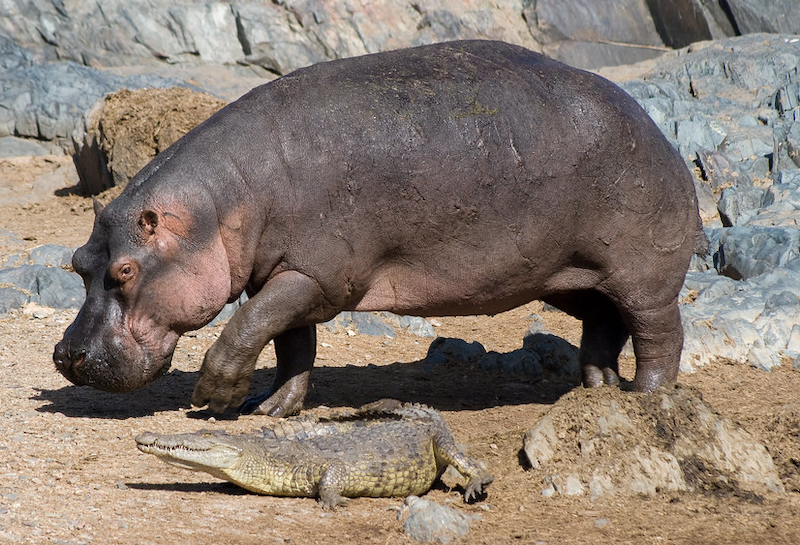
\includegraphics{images/sample-image.png}
\caption{\label{fig:sample-image}Leyenda con enlaces en formato \emph{Markdown}, pero sin la posibilidad de establecer notas al pie}
\end{figure}

\begin{verbatim}
...como se muestra en la Figura \\ref{fig:sample-image}.

Leyenda con enlaces en formato \emph{Markdown}, pero sin la posibilidad de establecer notas al pieLeyenda con enlaces en formato _Markdown_, pero sin la posibilidad de establecer notas al pie

  (```){r sample-image, fig.cap="Leyenda con enlaces en formato \emph{Markdown}, pero sin la posibilidad de establecer notas al pie"}
    knitr::include_graphics("images/sample-image.png")
  (```)

* los paréntesis son ilustrativos y se tienen que eliminar para que el fragmento de código funcione
\end{verbatim}

\hypertarget{demostraciuxf3n-fragmento-de-cuxf3digo-de-r-para-iframe-en-html-e-imagen-estuxe1tica-en-pdf-odt-docx-y-md}{%
\subsection{\texorpdfstring{Demostración: fragmento de código de \emph{R} para iframe en HTML e imagen estática en PDF, ODT, DOCX y MD}{Demostración: fragmento de código de R para iframe en HTML e imagen estática en PDF, ODT, DOCX y MD}}\label{demostraciuxf3n-fragmento-de-cuxf3digo-de-r-para-iframe-en-html-e-imagen-estuxe1tica-en-pdf-odt-docx-y-md}}

\ldots como se muestra en la Figura \ref{fig:sample-map}.



\begin{figure}
\centering

\includegraphics{images/sample-map.pdf}
\caption{\label{fig:sample-map}Explorar el mapa interactivo de \href{https://www.openstreetmap.org/note/3023469}{OSM}. Les lectorxs de ediciones que no sean HTML van a poder verlo de forma estática.}
\end{figure}

\begin{verbatim}
...como se muestra en la Figura \\ref{fig:sample-map}.

Explorar el mapa interactivo de \href{https://www.openstreetmap.org/note/3023469}{OSM}. Les lectorxs de ediciones que no sean HTML van a poder verlo de forma estática. Explorar el mapa interactivo de [OSM](https://www.openstreetmap.org/note/3023469). Les lectorxs de ediciones que no sean HTML van a poder verlo de forma estática.

(```){r sample-map, fig.cap="Explorar el mapa interactivo de \href{https://www.openstreetmap.org/note/3023469}{OSM}. Les lectorxs de ediciones que no sean HTML van a poder verlo de forma estática."}
if(knitr::is_html_output(excludes="markdown")) knitr::include_url("https://www.openstreetmap.org/note/3023469", height = "375px") else knitr::include_graphics("images/sample-map.png")
(```)
\end{verbatim}

\hypertarget{demostraciuxf3n-fragmento-de-cuxf3digo-de-r-para-gif-animado-en-html-e-imagen-estuxe1tica-en-pdf-odt-docx-y-md}{%
\subsection{\texorpdfstring{Demostración: fragmento de código de \emph{R} para GIF animado en HTML e imagen estática en PDF, ODT, DOCX y MD}{Demostración: fragmento de código de R para GIF animado en HTML e imagen estática en PDF, ODT, DOCX y MD}}\label{demostraciuxf3n-fragmento-de-cuxf3digo-de-r-para-gif-animado-en-html-e-imagen-estuxe1tica-en-pdf-odt-docx-y-md}}

\ldots como se muestra en la Figura \ref{fig:sample-gif}.



\begin{figure}
\centering
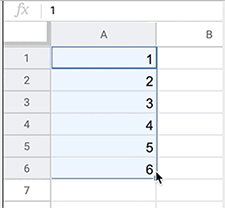
\includegraphics{images/sample-gif.pdf}
\caption{\label{fig:sample-gif}Ver un \href{https://etalii.github.io/tepepub/images/sample.gif}{GIF animado}. Les lectorxs de ediciones que no sean HTML van a poder verlo de forma estática}
\end{figure}

\begin{verbatim}
...como se muestra en la Figura \\ref{fig:sample-gif}.

Ver un \href{https://etalii.github.io/tepepub/images/sample.gif}{GIF animado}. Les lectorxs de ediciones que no sean HTML van a poder verlo de forma estática Ver un [GIF animado](https://etalii.github.io/tepepub/images/sample.gif). Les lectorxs de ediciones que no sean HTML van a poder verlo de forma estática

(```){r sample-gif, fig.cap="Ver un \href{https://etalii.github.io/tepepub/images/sample.gif}{GIF animado}. Les lectorxs de ediciones que no sean HTML van a poder verlo de forma estática"}
if(knitr::is_html_output(excludes="markdown")) knitr::include_url("images/sample-gif.gif", height = "250px") else knitr::include_graphics("images/sample-gif.png")
(```)
\end{verbatim}

\hypertarget{demostraciuxf3n-fragmento-de-cuxf3digo-de-r-para-incrustar-video-en-html-e-imagen-estuxe1tica-en-pdf-odt-docx-y-md}{%
\subsection{\texorpdfstring{Demostración: fragmento de código de \emph{R} para incrustar video en HTML e imagen estática en PDF, ODT, DOCX y MD}{Demostración: fragmento de código de R para incrustar video en HTML e imagen estática en PDF, ODT, DOCX y MD}}\label{demostraciuxf3n-fragmento-de-cuxf3digo-de-r-para-incrustar-video-en-html-e-imagen-estuxe1tica-en-pdf-odt-docx-y-md}}

Para esto hay que asegurarse de usar el enlace de inserción de \emph{YouTube}, \emph{Vimeo} o cualquiera sea la fuente del video en la web.

\ldots como se muestra en el Video \ref{fig:sample-video}



\begin{figure}
\centering
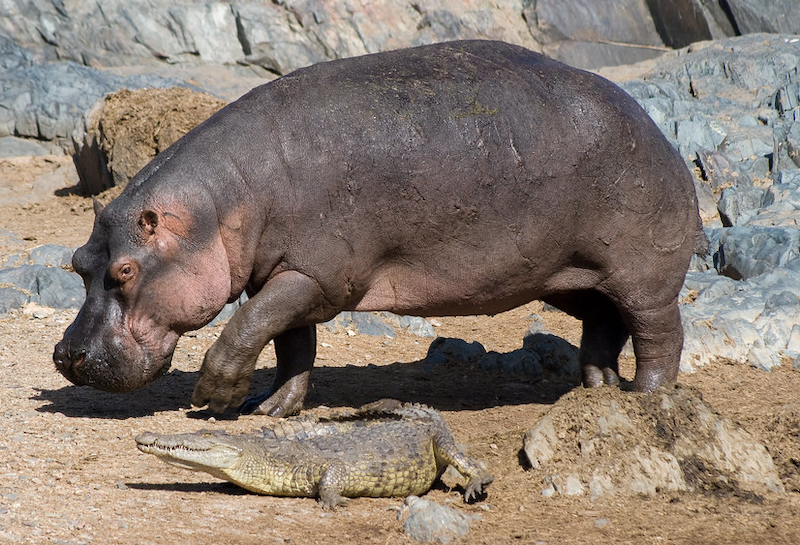
\includegraphics{images/sample-image2.png}
\caption{\label{fig:sample-video}Ver un \href{https://www.youtube.com/watch?v=dVqVscgwSpw}{video en YouTube}. Les lectorxs de ediciones que no sean HTML van a poder verlo de forma estática}
\end{figure}

\begin{verbatim}
...como se muestra en el Video \\ref{fig:sample-video}

Ver un \href{https://www.youtube.com/watch?v=dVqVscgwSpw}{video en YouTube}. Les lectorxs de ediciones que no sean HTML van a poder verlo de forma estática Ver un [video en YouTube](https://www.youtube.com/watch?v=dVqVscgwSpw). Les lectorxs de ediciones que no sean HTML van a poder verlo de forma estática

(```){r sample-video, fig.cap="Ver un \href{https://www.youtube.com/watch?v=dVqVscgwSpw}{video en YouTube}. Les lectorxs de ediciones que no sean HTML van a poder verlo de forma estática"}
if(knitr::is_html_output(excludes="markdown")) knitr::include_url("https://www.youtube.com/embed/dVqVscgwSpw") else knitr::include_graphics("images/sample-image2.png")
(```)
\end{verbatim}

\hypertarget{manejo-de-tablas-en-formato-markdown}{%
\subsection{\texorpdfstring{Manejo de tablas en formato \emph{Markdown}}{Manejo de tablas en formato Markdown}}\label{manejo-de-tablas-en-formato-markdown}}

La creación de tablas en formato Markdown se puede gestionar mediante \href{https://www.tablesgenerator.com/markdown_tables}{\emph{Tables Generator}} que además de producir buenos resultados para HTML, PDF, odt, doc y \emph{Markdown} permite importar datos de tablas en formato CSV.

El código de la tabla \emph{Markdown} que se muestra a continuación se tiene que agregar a la numeración automática (Tabla x) en HTML, PDF, odt y doc (Ver Tabla \ref{tab:left-table}).

\begin{longtable}[]{@{}
  >{\raggedright\arraybackslash}p{(\columnwidth - 4\tabcolsep) * \real{0.56}}
  >{\raggedright\arraybackslash}p{(\columnwidth - 4\tabcolsep) * \real{0.22}}
  >{\raggedright\arraybackslash}p{(\columnwidth - 4\tabcolsep) * \real{0.22}}@{}}
\caption{\label{tab:left-table} Contenido alineado a izquierda. Recordar dejar una fila en blanco entre los encabezados/ nombres de las columnas y el contenido}\tabularnewline
\toprule
Un encabezado muy muy largo & Encabezado corto & Encabezadito \\
\midrule
\endfirsthead
\toprule
Un encabezado muy muy largo & Encabezado corto & Encabezadito \\
\midrule
\endhead
Contenido alineado a la izquierda & número/ texto & número/ texto \\
Se pueden usar guines para obtener columnas más grandes & número/ texto & número/ texto \\
\bottomrule
\end{longtable}

Se compone así:

\begin{verbatim}
...(Ver Tabla \\ref{tab:left-table}).

Table: \label{tab:left-table} Contenido alineado a izquierda. Recordar dejar una fila en blanco entre los encabezados/ nombres de las columnas y el contenido

| Un encabezado muy muy largo | Encabezado corto | Encabezadito |
|:---------|:---|:---|
| Contenido alineado a la izquierda | número/ texto | número/ texto |
| Se pueden usar guines para obtener columnas más grandes | número/ texto | número/ texto |
\end{verbatim}

Si queremos que el contenido esté alineado a la derecha como se muestra en la Tabla \ref{tab:right-table}

Tabla: \label{tab:right-table} Contenido alineado a la derecha. Recordar dejar una fila en blanco entre los encabezados/ nombres de las columnas y el contenido

\begin{longtable}[]{@{}
  >{\raggedleft\arraybackslash}p{(\columnwidth - 4\tabcolsep) * \real{0.33}}
  >{\raggedleft\arraybackslash}p{(\columnwidth - 4\tabcolsep) * \real{0.33}}
  >{\raggedleft\arraybackslash}p{(\columnwidth - 4\tabcolsep) * \real{0.33}}@{}}
\toprule
Encabezado1 & Encabezado2 & Encabezado3 \\
\midrule
\endhead
123 & 456 & 789 \\
Contenido alineado a la derecha & número/ texto & número/ texto \\
la misma cantidad de guiones & entre las columnas de la línea en blanco & garantiza mismo tamaño de columnas \\
\bottomrule
\end{longtable}

Se debe componer así:

\begin{verbatim}
...como se muestra en la Tabla \\ref{tab:right-table}

Tabla: \label{tab:right-table} Contenido alineado a la derecha. Recordar dejar una fila en blanco entre los encabezados/ nombres de las columnas y el contenido

| Encabezado1 | Encabezado2 | Encabezado3 |
|-----:|-----:|-----:|
| 123 | 456 | 789 |
| Contenido alineado a la derecha | contenido numérico | contenido numérico |
| la misma cantidad de guiones | entre las columnas de la línea en blanco | garantiza mismo tamaño de columnas |
\end{verbatim}

\hypertarget{compilar}{%
\chapter{Compilar}\label{compilar}}

\hypertarget{distintos-formatos-en-un-solo-paso}{%
\section{Distintos formatos en un solo paso}\label{distintos-formatos-en-un-solo-paso}}

Para compilar el libro/ publicación en múltiples formatos (HTML, \emph{LaTeX}/ PDF, odt, doc y Epub) y en un solo paso, se puede llamar la función \texttt{bookdown::render\_book()} desde la línea de comandos de \emph{R} o hacer \emph{click} en el botón \texttt{Build\ Book} del panel \texttt{Build} en \emph{RStudio}.

Por otro lado, los formatos de salida se configuran en el archivo \texttt{\_output.yml} del proyecto. En el caso que, por ejemplo, se desee compilar una publicación en los formatos libro de \emph{git} (\emph{gitbook}), HTML, \emph{LaTeX}/ PDF y Epub, dicho archivo YAML se debe configurar de la siguiente forma:

\begin{verbatim}
output:
  bookdown::gitbook:
    css: style.css
    repo: https://github.com/etalii/tepepub
    config:
      toc:
        before: |
          <li> </li>
        after: |
          <li> </li>
      download: ["pdf", "epub"]
  bookdown::pdf_book:
    includes:
      in_header: preamble.tex
    latex_engine: xelatex
    citation_package: natbib
    keep_tex: yes
  bookdown::html_book
  bookdown::epub_book: default
\end{verbatim}

\hypertarget{uso-del-formato-condicional}{%
\section{Uso del formato condicional}\label{uso-del-formato-condicional}}

El formato condicional ofrece la opción de mostrar texto o imágenes en algunas ediciones de la publicación, pero no en otras. A continuación, se muestran varias formas de utilizar el formato condicional:

\begin{itemize}
\item
  Insertar un comentario de código HTML \texttt{\textless{}!\ -\ comentario\ -\textgreater{}} en el archivo \texttt{.Rmd} para ocultar algunas líneas de texto. Esto aparece como texto comentado en los formatos HTML y .md, por ende, no se muestra en el navegador HTML y no aparece de ninguna manera en los formatos PDF o .doc .
\item
  Adecuar la salida condicional a diferentes publicaciones mediante la función del paquete de \emph{R} \texttt{is\_\ {[}html\ /\ latex{]}\ \_output} que permite, por ejemplo, que el texto sea visible en la edición HTML, pero no en la edición PDF o viceversa.
\item
  Personalizar el código de las hojas de estilo en \emph{CSS} ( \texttt{style.css} ) de la publicación web.
\item
  Agregar encabezados, pies de página y bajadas al texto en las versiones HTML o \emph{LaTeX}.
\item
  Compilar diferentes versiones de la publicación en HTML y \emph{LaTeX} / PDF que se compongan de los mismos capítulos/ secciones en distinto órden, mediante la enumeración diferencial en el archivo\texttt{\_bookdown.yml}. De esta manera es posible publicar todos los capítulos / secciones para la versión HTML, mientras que solamente se compilen los capítulos seleccionados en el PDF:
\end{itemize}

\begin{verbatim}
# cuando se compilan todos los capítulos para un libro/ publicación HTML hay que comentarlos todos, mientras que se tiene que  eliminar el comentario para omitir los capítulos que no se enumeran a continuación de las versiones PDF y _Markdown_ para ORM


# rmd_files: [
#   "index.Rmd",
#   "0.0-introduction.Rmd",
#   "01-choose.Rmd",
#   "02-spreadsheet.Rmd",
#   "03-find.Rmd",
#   "04-clean.Rmd",
#   "05-comparisons.Rmd",
#   "06-chart.Rmd",
#   "07-map.Rmd",
#   "08-table.Rmd",
#   "09-embed.Rmd",
#   "10-github.Rmd",
#   "11-chartcode.Rmd",
#   "12-leaflet.Rmd",
#   "13-transform.Rmd",
#   "14-detect.Rmd",
#   "15-story.Rmd",
#   "16-fix.Rmd",
#   "21-references.Rmd"
# ]
\end{verbatim}

\hypertarget{publicar}{%
\chapter{Publicar}\label{publicar}}

\hypertarget{github-y-el-cuxf3digo-como-infraestructura}{%
\section{\texorpdfstring{\emph{Github} y el código como infraestructura}{Github y el código como infraestructura}}\label{github-y-el-cuxf3digo-como-infraestructura}}

Si bien \emph{Bookdown} no requiere el uso de \emph{GitHub}, este flujo de trabajo integra \emph{Bookdown} y \emph{GitHub} mediante la función \texttt{bookdown::gitbook} y el archivo de salida \texttt{gitbook} para generar una publicación o libro web. Para ello hace falta:

\begin{enumerate}
\def\labelenumi{\arabic{enumi}.}
\item
  Crear una cuenta en \emph{Git} y/o registrarse en \emph{GitHub}
\item
  Una vez iniciada la sesión en una cuenta de \emph{GitHub} hay que dirigirse al \href{https://github.com/yihui/bookdown-minimal}{repositorio mínimo de bookdown} , ``forkear'' (aplicar el comando/ evento \texttt{fork} de \emph{git}) y crear una copia.
\item
  Instalar un cliente de escritorio para \emph{Git}, puede ser \href{https://desktop.github.com}{GitHub Desktop} o \href{https://www.gitkraken.com/}{GitKraken} . Éste se va usar para transferir archivos entre el repositorio de \emph{GitHub} en la nube y la computadora local desde donde se compone la publicación. Si bien los desarrolladores de software pueden preferir acceder a \emph{GitHub} desde la línea de comandos de la terminal, los clientes de escritorio pueden proporcionar un acceso más sencillo.
\item
  En \emph{RStudio}, en la esquina superior derecha, seleccionar Project \textgreater{} Open Project para abrir la carpeta \texttt{bookdown-minimal} de forma local \href{images/project-open.png}{ver captura de pantalla}.
\item
  En \emph{RStudio}, abrir el archivo \texttt{index.Rmd} y realizar algunas ediciones simples en el texto. Por ejemplo, eliminar el símbolo de \emph{hashtag} ( \# ) en la línea 8 para ``descomentar'' y activar la opción de la salida PDF y guardar las ediciones \href{images/edit-book.png}{ver captura de pantalla}.
\item
  En \emph{RStudio}, en la esquina superior derecha, seleccionar la pestaña \texttt{Build}, seleccionar la opción \texttt{Build\ Book} y elegir \texttt{All\ Formats} para crear, tanto la edición web estática de estilo \emph{gitbook}, como la salida en PDF.
\item
  Si \emph{RStudio} compila con éxito ambas versiones del libro, la salida se guardará en la subcarpeta \texttt{\_book}. Además, el navegador interno de \emph{RStudio} debería abrir automáticamente la edición web.
\item
  Si durante la compilación se generó algún tipo de error, los mensajes de error van a aparecer en rojo en el visor de \emph{RStudio} de la pestaña \texttt{Build}, lo que puede requerir depurar los errores y eliminar los archivos temporales según las instrucciones \href{images/build-book.png}{ver captura de pantalla}.
\end{enumerate}

Sugerencia: para futuras sesiones de \emph{RStudio} que se abran, es recomendable seleccionar la pestaña \texttt{Packages} y hacer click en \texttt{Update} para mantener \emph{Bookdown} y otros paquetes de software actualizados
\href{images/update-packages.png}{ver captura de pantalla}.

\begin{enumerate}
\def\labelenumi{\arabic{enumi}.}
\setcounter{enumi}{8}
\item
  Al cerrar el proyecto y salir de \emph{RStudio}, el siguiente conjunto de pasos se centrará en enviar la publicación al repositorio de \emph{GitHub} utilizando el cliente de escritorio.
\item
  Una vez abierto el cliente de escritorio, navegar hasta la carpeta local del proyecto, escribir un resumen rápido para confirmar (o guardar) los cambios que se realizaron anteriormente en la rama maestra y enviar esta versión al repositorio de \emph{GitHub} en la nube.
\item
  Dirigirse al repositorio de \emph{GitHub} del proyecto con un navegador web.
\item
  En el repositorio de \emph{GitHub}, seleccionar \emph{Settings} (Configuración) y en la sección \emph{GitHub Pages} (Páginas de GitHub) -que es un servicio de alojamiento web gratuito para publicar código y publicaciones/ libros en la web pública-, donde dice \texttt{Source} hay que cambiar de \texttt{None} (Ninguna) a \texttt{Main} (Principal), mantener la opción \texttt{default\ /root} (predeterminada / raíz) y presionar \texttt{Save} (Guardar).
\item
  En la sección \emph{GitHub Pages} la dirección web del sitio publicado debería ser similar a: \texttt{https://NOMBREDEUSUARIX.github.io/nombre-del-proyecto}
\item
  Copiar la dirección web, pegarla en una nueva ventana o pestaña del navegador y al final, agregar \texttt{\_book} / \texttt{index.html}. La publicación está configurada de forma predeterminada para almacenar todas las ediciones web y PDF en la subcarpeta \texttt{\_book}, con \texttt{index.html} como página de inicio. Por lo tanto, la dirección web completa en la nueva pestaña del navegador debería ser similar a: \texttt{https://NOMBREDEUSUARIX.github.io/nombre-del-proyecto/\_book/index.html} .
\end{enumerate}

Otra sugerencia: es posible que haya que esperar hasta un minuto para que las ediciones hechas en el repositorio de \emph{GitHub} en la nube, aparezcan en la dirección web del proyecto. Además, después de esperar a que la web realice los cambios, es recomendable asegurarse de ``forzar la recarga'' o ``actualizar por completo'' el navegador web para que la versión de la vista que se obtiene, se actualice directamente desde el servidor de \emph{GitHub} y no desde la memoria \emph{caché} interna del navegador.

\hypertarget{el-libro-publicaciuxf3n-web-y-los-archivos-de-salida}{%
\section{El libro/ publicación web y los archivos de salida}\label{el-libro-publicaciuxf3n-web-y-los-archivos-de-salida}}

La principal diferencia entre renderizar un libro/ publicación web usando \emph{Bookdown} y renderizar un único documento \texttt{.rmd} usando \emph{R Markdown}, a HTML, es que para el libro/ publicación web se generarán varias páginas HTML de forma predeterminada, un archivo HTML por capítulo. Esto hace que sea más fácil marcar un capítulo determinado o compartir su URL y que resulte más rápido cargar un libro/ publicación web en el navegador. Hay distintos estilos para la salida HTML, pero en este trabajo se presenta el estilo desarrollado por \emph{GitBook}, con algunas \emph{features} aportadas por \emph{Bookdown}..

La interfaz de navegación \citep{manovichLenguajeNuevosMedios2006} de \href{https://www.gitbook.com}{\emph{GitBook}} presenta el contenido en bloques \citep{seminariopublicacionesdigitalesUnidadParte2021b}, de forma que consiste en una barra lateral (\emph{sidebar}) a la izquierda, que muestra la tabla de contenidos y el cuerpo principal de la publicación a la derecha. Esta barra se puede colapsar en caso de que se quiera ampliar la vista del contenido. Por otro lado, el diseño tiene comportamiento responsive, es decir, responde al tamaño de la ventana. Por ejemplo, los botones de navegación se muestran a la izquierda/ derecha del cuerpo de la publicación cuando la ventana es lo suficientemente ancha y se contraen en la parte inferior cuando la ventana es estrecha, de forma de dar a les lectorxs más campo horizontal para leer.

La forma más fácil de generar un \emph{gitbook} es usar el asistente de proyectos (\emph{Wizard}) de \emph{RStudio} (File \textgreater{} New Project \textgreater{} New Directory \textgreater{} Book project using bookdown) y seleccionar \emph{gitbook} en el menú desplegable (ver Figura \ref{fig:new-bs4-book} ).

\begin{figure}

{\centering 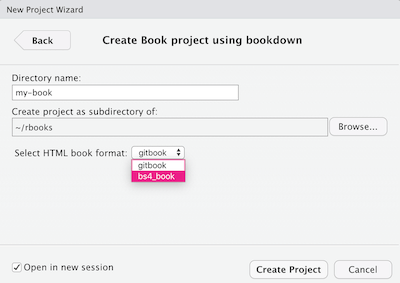
\includegraphics{images/new-bs4-book} 

}

\caption{Captura de pantalla del asistente de proyectos de RStudio para crear un nuevo proyecto de libro/ publicación.}\label{fig:new-bs4-book}
\end{figure}

Lo mismo se puede lograr desde la consola de \emph{R} mediante el comando \texttt{bookdown::create\_gitbook()} pero este método es mucho menos accesible a personas que carezcan o cuenten con poca predisposición para trabajar con herramientas avanzadas de programación.

Sobre la base de lo que ofrece la versión nativa de \emph{GitBook}, \emph{Bookdown} cuenta con una serie de mejoras. La más importante consiste en el uso de \emph{R Markdown} (\emph{Rmd}) v2, basado en \emph{Pandoc}.

La interfaz del libro/ publicación web, además, hereda de \emph{GitBook} una barra de herramientas (\emph{toolbar}) (ver Figura \ref{fig:gitbook} ) en la parte superior de cada página que permite cambiar dinámicamente la configuración de la visualización, botón de búsqueda, descarga de otros formatos de salida (LaTex, pdf, epub y mobi) y compartir en redes sociales ( \emph{Facebook}, \emph{Twitter} e \emph{Instapaper} por ejemplo). Asímismo, la opción de la barra de herramientas tiene una posición de sub-opción que puede tomar valores fijos o estáticos. El valor predeterminado es que la barra de herramientas quede fija (\emph{sticky}) en la parte superior de la página, por lo que incluso si se desplaza hacia abajo, la barra de herramientas seguirá estando visible.

\begin{figure}

\includegraphics[width=1\linewidth]{images/gitbook} \caption{barra de herramientas del libro/ publicación web. }\label{fig:gitbook}
\end{figure}

Por otro lado, en el archivo \texttt{\_bookdown.yml} se pueden configurar un conjunto de opciones de nivel superior y metadatos que se pueden pasar a la plantilla HTML del libro / publicación web a través de \emph{Pandoc}. Es posible que no tengan efectos visibles en la salida HTML, pero pueden ser útiles cuando dicha salida se implementa como sitio web. Estas opciones incluyen:

\begin{itemize}
\item
  \texttt{description:} una cadena de caracteres que se escribirá en el atributo \texttt{content} de la etiqueta \texttt{\textless{}meta\ name="description"\ content=""\textgreater{}} en el encabezado HTML (si falta, se usará el título del libro). Configurar esta opción tiene importancia para la optimización de motores de búsqueda (SEO).
\item
  \texttt{url:} la \emph{URL} del sitio web del libro, por ejemplo, \url{https://etalii.github.io/tepepub/}
\item
  \texttt{github-repo:} El repositorio de \emph{GitHub} del libro/ publicación en la forma usuarie/repo.
\item
  \texttt{cover-image:} la ruta a la imagen de portada del libro/ publicación.
\item
  \texttt{favicon:} Una ruta al ícono que se muestra en la barra de direcciones del navegador o frente al título de la página en la pestaña si el navegador admite pestañas.
\end{itemize}

A continuación se muestra a modo de ejemplo la lista completa de estas opciones de configuración de metadatos YAML:

\begin{verbatim}
title: "An Awesome Book"
author: "John Smith"
description: "This book introduces the ABC theory, and ..."
url: 'https\://bookdown.org/john/awesome/'
github-repo: "john/awesome"
cover-image: "images/cover.png"
favicon: "favicon.ico"
\end{verbatim}

Notar que un efecto deseable de configurar la descripción y la imagen de portada es que cuando se comparta el enlace del libro/ publicación web en los sitios de redes sociales, el enlace puede expandirse automáticamente a una tarjeta con la imagen de portada y la descripción del libro/ publicación.

Finalmente, al pie de la barra de contenidos se encuentra el link al repositorio de \emph{GitHub} donde se encuentran los archivos fuente en formato \emph{Rmd}.

\hypertarget{discusiuxf3n-y-conclusiuxf3n}{%
\chapter{Discusión y conclusión}\label{discusiuxf3n-y-conclusiuxf3n}}

Desarrollar un sistema de gestión editorial de forma digital, descentralizado, distribuido y en la nube; desde la recepción del original hasta la publicación final, la difusión y la comercialización; sin duda requiere de mucho más que simplemente desarrollar un flujo de trabajo a través del cual un mismo contenido puede culminar en distintos archivos de salida, formatos, publicaciones y soportes. Pero es un comienzo. Para escalar dicho desarrollo hay que armar un plan editorial y disponer de un esquema organizacional integrado que permita llevar a cabo procesos de toma de decisiones exhaustivos respecto a la organización de las publicaciones \citep{seminariopublicacionesdigitalesUnidadParte}, las comunidades lectoras a las que se dirige, el vínculo con ellas, la promoción de ventas y los medios, tecnologías y estrategias de financiamiento.

Si bien en este trabajo no se analizó el aspecto del sistema de gestión editorial, las herramientas que se comentaron aportan medios simbólicos y tecnológicos para dicho desarrollo. En particular, vale la pena destacar la importancia que tiene la incorporación de \emph{software} de control de versiones (\emph{Git}) y sobre todo, de las funciones que plataformas como \emph{GitHub} y \href{https://about.gitlab.com/}{\emph{GitLab}} hacen posibles; entre ellas, \href{https://docs.github.com/en}{\emph{issues}, \emph{boards} y \emph{milestones}}. Funciones complementarias a otras ya mencionadas, como disponer de una plataforma como infraestructura para el trabajo colaborativo y la gestión de la memoria editorial, todo en un mismo repositorio en la nube.

Como se mencionó en la \protect\hyperlink{intro}{Introducción}, el lenguaje de programación \emph{R} -utilizado para llevar a cabo este desarrollo-, suele emplearse para análisis estadístico y por lo tanto, \emph{Bookdown} suele estar orientado a la publicación de trabajos académicos y la documentación en el campo del desarrollo de \emph{software}. De ahí se desprenden dos cuestiones: por un lado, la importancia de incorporar a conciencia ciertas características propias de esos contextos productivos a cualquier flujo de trabajo que se base en dichas tecnologías; y por otro lado, la necesidad de repensar relaciones definibles de forma hipertextual, hipermedial y transmedial \citep{seminariopublicacionesdigitalesUnidadParte2021}, y que esto a su vez se transforme en casos de uso y herramientas capitalizables en concreto, por ejemplo, en el desarrollo de temas y plantillas específicos para distintos géneros editoriales y literarios. Cuestión que remite a las formas de apropiación (Idem) y relación entre les lectorxs y el contenido, y que no está saldada hasta que esa apropiación se vuelve efectiva por parte de una comunidad de desarrolladorxs, editorxs, autorxs y lectorxs.

En relación a lo anterior, es posible identificar que \emph{Git} puede tener cierto valor estratégico, tanto en lo que respecta a la gestión de las redes sociales (referido a las redes que conectan personas, organizaciones e instituciones y no a las plataformas de medios sociales como fb, tw e ig), como a la capacidad técnica de administrar procesos editoriales colaborativos: otorgar permisos diferentes a distintxs usuaries, recibir artículos, revisiones y comentarios, hacer evaluaciones (tipo \emph{peer review}) y aceptar o rechazar cambios \footnote{Para conocer cómo funciona el comando/ evento \emph{Pull request}/ \emph{Merge request} y su aplicación en el desarrollo de proyectos colaborativos, ver: \url{https://docs.github.com/en/pull-requests}}. A su vez, hace falta extraer sentidos editoriales de dicha identificación, para así generar un tipo de mirada disciplinar a partir de los aportes e intereses de la comunidad de desarrollo vinculada a \emph{Bookdown}.

Uno de esos emergentes es la potencialidad que tiene la combinación de \emph{R}, \emph{Bookdown} y \emph{Git} para la gestión de publicaciones de actualización periódica, publicaciones seriadas \citep{seminariopublicacionesdigitalesUnidadParte2021a} y publicaciones científicas, cuando las tecnologías son gestionadas por las comunidades de usuaries \footnote{Ver por ejemplo:\url{https://github.com/pkp/ojs}}. Así, de forma similar a lo propuesto por McLuhan \citep{marshallmcluhanComprenderMediosComunicacion1994} respecto a las prácticas de lectura y escritura; el acceso al conocimiento y la posibilidad de apropiación de las tecnologías libres y de código abierto, son las condiciones materiales que hacen posible que les usuaries se involucren de forma activa en el campo del desarrollo de \emph{software}. Por lo tanto, dichas condiciones también pueden posibilitar experiencias similares de transformación en otros campos de producción de conocimiento. La cuestión sería entonces, si una vez generadas las condiciones sociales, simbólicas, materiales y tecnológicas, podrían replicarse fenómenos similares en las comunidades de editorxs, autorxs y lectorxs como un todo y en relación a las publicaciones digitales.

Por último, desde el punto de vista editorial, la edición electrónica como proceso no está del todo concluida sin la disposición pública de la publicación en alguna plataforma de comercialización. Es decir que, para completar el flujo de trabajo, queda pendiente la integración a una tienda virtual o servicio de \emph{ecommerce}. Este, siguiendo la filosofía de las licencias libres y las posibilidades que ofrecen las herramientas de desarrollo que constituyen los fragmentos de código de \emph{R} para adecuar el contenido a distintos formatos digitales, idealmente debería permitir administrar un sistema de previsualización y suscripción a distintos tipos de contenidos de una misma publicación.

Una opción para simplificar esa tarea puede ser \href{https://www.bookwire.es/}{\emph{Bookwire}} que permite llevar la publicación a centenares de tiendas electrónicas desde una sola plataforma. O alternativamente, implementar el uso de \href{https://docs.github.com/en/actions}{\emph{Actios} de \emph{GitHub}} en conjunto con \emph{GitHub Pages} para, en un mismo portal, integrar servicios de catálogo, gestión de existencias - stock, promoción de ventas, tienda y comercialización \citep{seminariopublicacionesdigitalesUnidad2021}.

Xie, Yihui. \emph{Bookdown: Authoring Books and Technical Documents with R Markdown}. Chapman \& Hall/CRC, 2018. \url{https://bookdown.org/yihui/bookdown/}.

Xie, Yihui, J. J. Allaire, and Garrett Grolemund. \emph{R Markdown: The Definitive Guide}. Chapman \& Hall/CRC, 2020. \url{https://bookdown.org/yihui/rmarkdown/}.

Xie, Yihui, Christophe Dervieux, and Emily Riederer. \emph{R Markdown Cookbook}. Chapman \& Hall/CRC, 2020. \url{https://bookdown.org/yihui/rmarkdown-cookbook/}.

  \bibliography{book.bib,packages.bib}

\end{document}
